\documentclass[10pt,journal]{IEEEtran}
\usepackage{graphicx}
\usepackage{amsmath}
\usepackage[hidelinks]{hyperref}
\graphicspath{{plots/}}

\title{FarmFederate --- Supplementary Figures}
\author{}
\date{}

\begin{document}
\maketitle

\noindent
Every figure here is generated from a completed run whose aggregate numbers are
already reported in the main paper: the aligned 222/74/75 crop--note support,
the clubbed centralized/federated sweep, the matched-setting standard tier
(50 rounds), the three-seed frozen-encoder federated runs, and the advisory
retrieval evaluation. Figures the main paper carries are not repeated. Plots
from the superseded pipelines that remain in the repository --- the
\texttt{rag\_01}--\texttt{rag\_06} series and the earlier five-class
crop-stress charts --- measure a different corpus and are deliberately
excluded.

\section{Encoders on the aligned support}

\begin{figure}[htbp]\centering

\includegraphics[width=\linewidth]{sfig01_aligned_encoders}
\caption{Validation and test accuracy for every encoder on the identical
222/74/75 support. Text systems are saturated; the spread lives on the image
side.}
\end{figure}

\begin{figure}[htbp]\centering

\includegraphics[width=0.72\linewidth]{sfig02_generalisation_gap}
\caption{Validation minus test accuracy per system. A large positive gap means
the configuration was chosen on 74 crops and did not transfer; ConvNeXT-tiny
and ViT-Base show the largest.}
\end{figure}

\section{Note sparsity, per encoder}

\begin{figure}[htbp]\centering

\includegraphics[width=0.72\linewidth]{sfig03_clubbed_text}
\caption{Text encoders as notes are deleted; solid centralized, dashed
federated. TF-IDF degrades most gracefully, which is the bag-of-words result
discussed in the main paper.}
\end{figure}

\begin{figure}[htbp]\centering

\includegraphics[width=0.72\linewidth]{sfig04_clubbed_multimodal}
\caption{Fusions as notes are deleted, same protocol. The fused systems hold
above their text parents once a quarter of the notes remain.}
\end{figure}

\section{Federated behaviour}

\begin{figure}[htbp]\centering

\includegraphics[width=\linewidth]{sfig05_alpha_sweep_splitters}
\caption{All five architectures across the four skews under both splitters. The
corrected class-wise splitter produces the intended label skew; the legacy
size-only splitter does not, so its curves are flat in $\alpha$.}
\end{figure}

\begin{figure}[htbp]\centering

\includegraphics[width=\linewidth]{sfig09_round_curves_by_skew}
\caption{Per-round convergence of the frozen-encoder systems at both skews,
three seeds. The band spans the observed seed range.}
\end{figure}

\begin{figure}[htbp]\centering

\includegraphics[width=0.72\linewidth]{sfig06_cost_pareto}
\caption{Analytic float32 uplink per client-round against accuracy at
$\alpha=1$. The image-only arm is the cheapest and the weakest; text-only
reaches the ceiling at 42.4\,MiB.}
\end{figure}

\begin{figure}[htbp]\centering

\includegraphics[width=0.72\linewidth]{sfig08_anticollapse}
\caption{Anti-collapse components under actual federation, concat model. No arm
collapses, so the stack is reported rather than claimed necessary.}
\end{figure}

\begin{figure}[htbp]\centering

\includegraphics[width=\linewidth]{sfig07_warmstart_fusion_seeds}
\caption{(a)~Warm versus cold initialization, per seed. Trained out to 50
rounds cold start is better at one seed and identical at the other, reversing
the eight-round result. (b)~Fusion variants across seeds.}
\end{figure}

\section{Advisory corpus}

\begin{figure}[htbp]\centering

\includegraphics[width=\linewidth]{sfig10_corpus_audit}
\caption{(a)~What the advisory corpus contains after de-duplication: 3000
annotation rows collapse to 673 unique observations over 131 distinct
sentences, 43 of which appear in more than one class. (b)~Class balance of the
unique observations.}
\end{figure}

\section{Figures cut from the main paper for space}

\begin{figure}[htbp]\centering
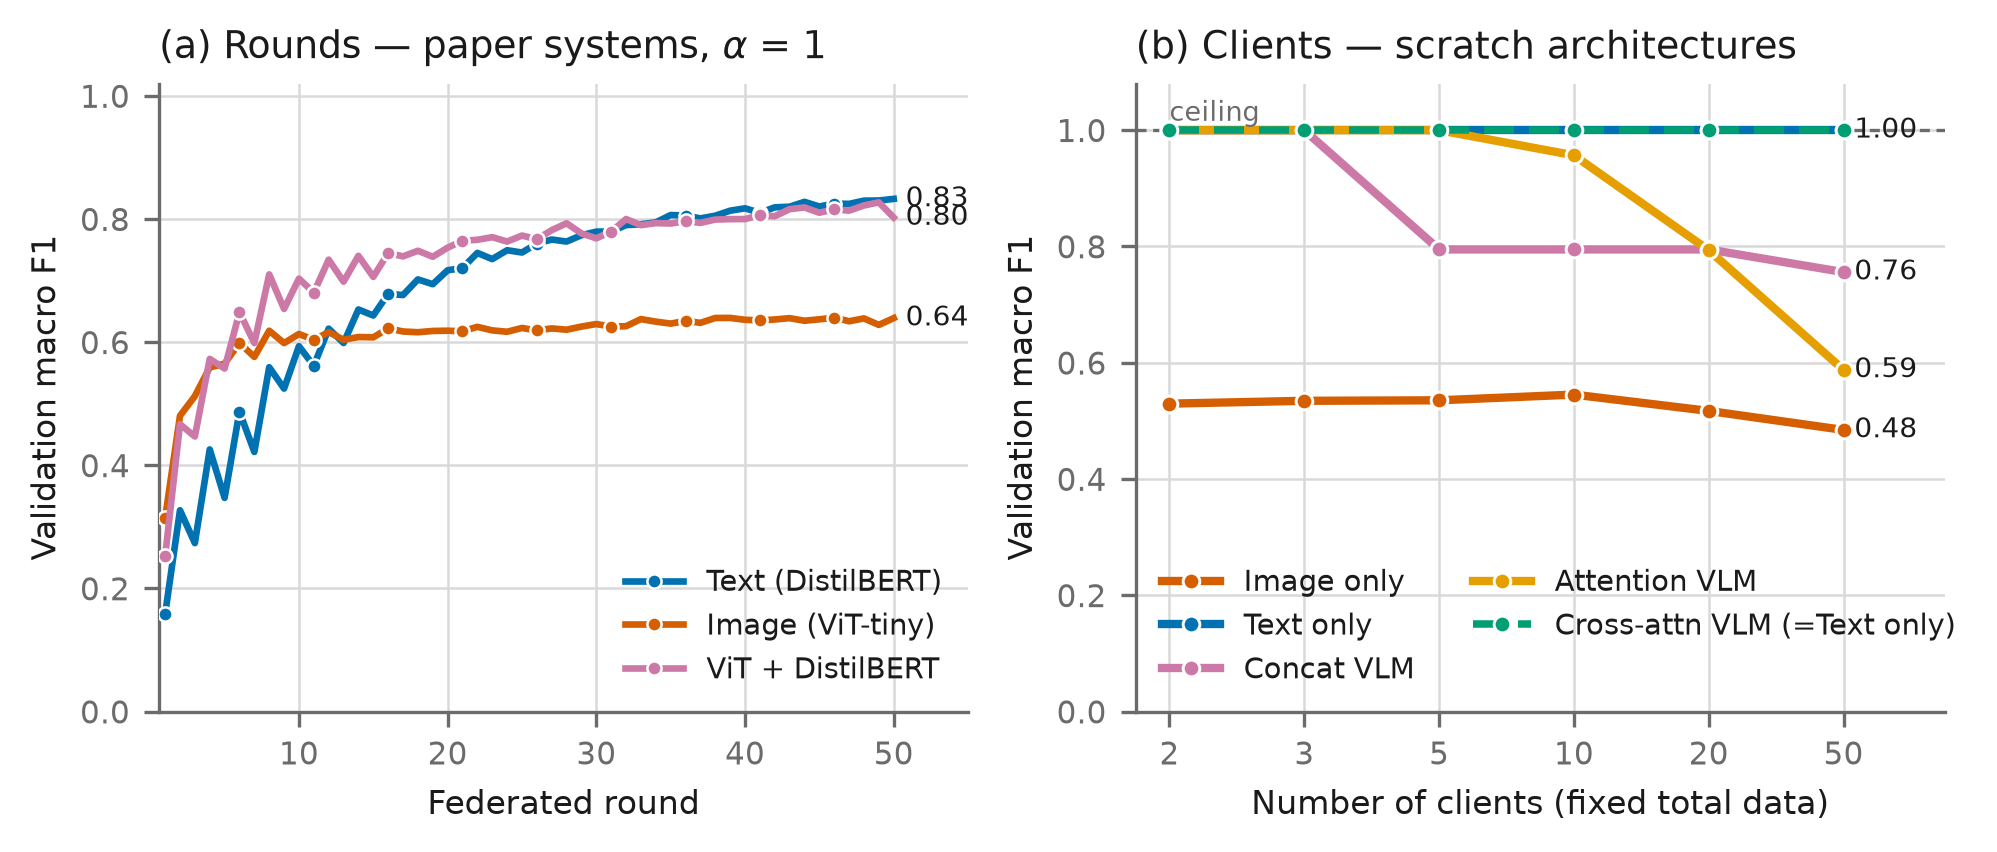
\includegraphics[width=\linewidth]{plot81_federated_rounds_clients}
\caption{Federated rounds and client scaling. Text overtakes fusion at round
33; text-only and cross-attention hold the ceiling to $K=50$.}
\end{figure}

\begin{figure}[htbp]\centering

\includegraphics[width=\linewidth]{plot86_aggregators}
\caption{Aggregators at $\alpha=0.1$ with the local-only control, and FedAvg
across skews. SCAFFOLD collapses to 0.088 on the attention VLM.}
\end{figure}

\begin{figure}[htbp]\centering

\includegraphics[width=\linewidth]{plot87_encoder_detail}
\caption{Per-encoder detail at 50\% note deletion, and the cost of federating
each system.}
\end{figure}

\begin{figure}[htbp]\centering

\includegraphics[width=\linewidth]{plot85_ladder_search}
\caption{Pipeline search size against accuracy, and the validation-to-test gap
it buys. Gates are hollow.}
\end{figure}

\begin{figure}[htbp]\centering
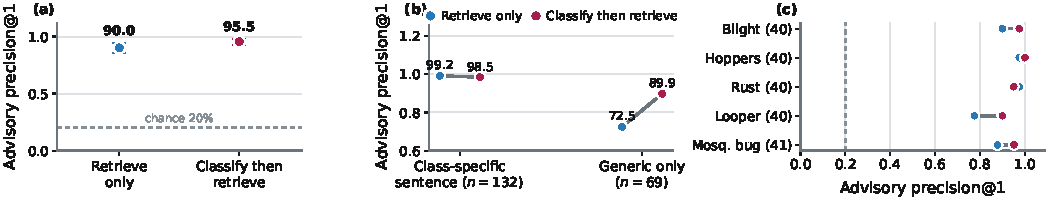
\includegraphics[width=0.86\linewidth]{plot80_advisory_retrieval}
\caption{Classify-Retrieve-Advise quality: headline precision@1, the
class-specific versus generic split, and the per-class breakdown.}
\end{figure}

\end{document}
